\section{Examples of Using Libvina}
\label{sec:adaption}

Programmers who apply our metaprogramming approach need to customize their
source code to utilize libvina.
%Libvina provides a group of \emph{concepts}
%to support transformations and expects programmrs to \emph{model} our
%template classes~\cite{tempmetaprog}. 
In the following, we describe two examples 
to illustrate the usage of our template library. 


\subsection{Example I: Hierarchy Pattern}

\begin{figure}[hbt]
  \inputsrc{sgemm.cc}
  \caption{Source code of matrix multiplication (class SGEMM) using hierarchy pattern.}
  \label{fig:sgemm}
\end{figure}

\reffig{sgemm} is the source code for matrix multiplication by adapting \code{TF\_hierarchy}
to implement a \emph{Divide-and-Conquer} algorithm. Recall in Section~\ref{sect:tf} that
\code{TF\_hierarchy} invokes \code{TASK:inner} for recursion and \code{TASK::leaf}
for computing subtasks. In this example, these two functions are defined at line
22 and 52, respectively.

The call operator function at line 15 is the user interface for this matrix multiplication task.
Note inside the template class, data are manipulated using views, which are defined
at line 7-9.

Line 11 defines \code{SELF} as task's type. Then at line 12 \code{SELF} is used as
the template parameter \code{TASK} for \code{TF\_hierarchy}. Template parameter \code{PRED} 
at line 12 is a predicate, which is evaluated by \code{TF\_hierarchy} class 
using \code{ARG0} and \code{ARG1}.

Inside function \code{inner}, lines 24-26 define size-reduced classes after dividing the task. 
Lines 28-44 describe a lambda expression~\cite{cpplambda} to perform a MapReduce-style computation.
Line 30 defines temporary matrices.
First, lambda $m$ computes $n$-th temporary sub-matrix, where line 40 computes
$K$ temporary matrices in parallel. Then, lines 42-43 reduces these
$K$ temporary matrices to obtain sub-matrix of row $i$, column $j$. 
Finally, lines 47-48 computes all sub-matrices in parallel.

%Line 30$\sim$32 of \reffig{sgemm} generate subviews by calling functions.

\reffig{mmexample} is a sample execution graph of \code{SGEMM},
where $M=P=N=4096$ and $k=2$.



%To leverage static information, libvina need to
%associate template parameters with ADTs' parameters. For example, 
%Matrix class cantains 3 template paramters: type, the number of
%row, the number of column. A definition of Matrix is at line 26 of
%\reffig{sgemm}. 


%\reffig{mmexample} illustrates ...

%Programmers using our template-based programming model are free to
%choose ways to parallelize tasks. An example of applying 
%Sequoia's programming model is shown in Fig.~\ref{fig:mmexample}. 
%\textit{sgemm} is a task to perform matrix-mulitplication. 
%We can apply a TF class dedicated to hierarchical division.  \reffig{sgemm}
%illustrates the adaption. As a reuslt, we
%implement the straightforward \emph{Divide-and-Conquer} algorithm for
%sgemm, which divides a matrix into K*K
%submatrices, computes them recursively, and reduces the results for
%each division.
%The control flow of source transformation is programmed
%using template metaprogramming inside of the TF class. 

\begin{figure}[htb]
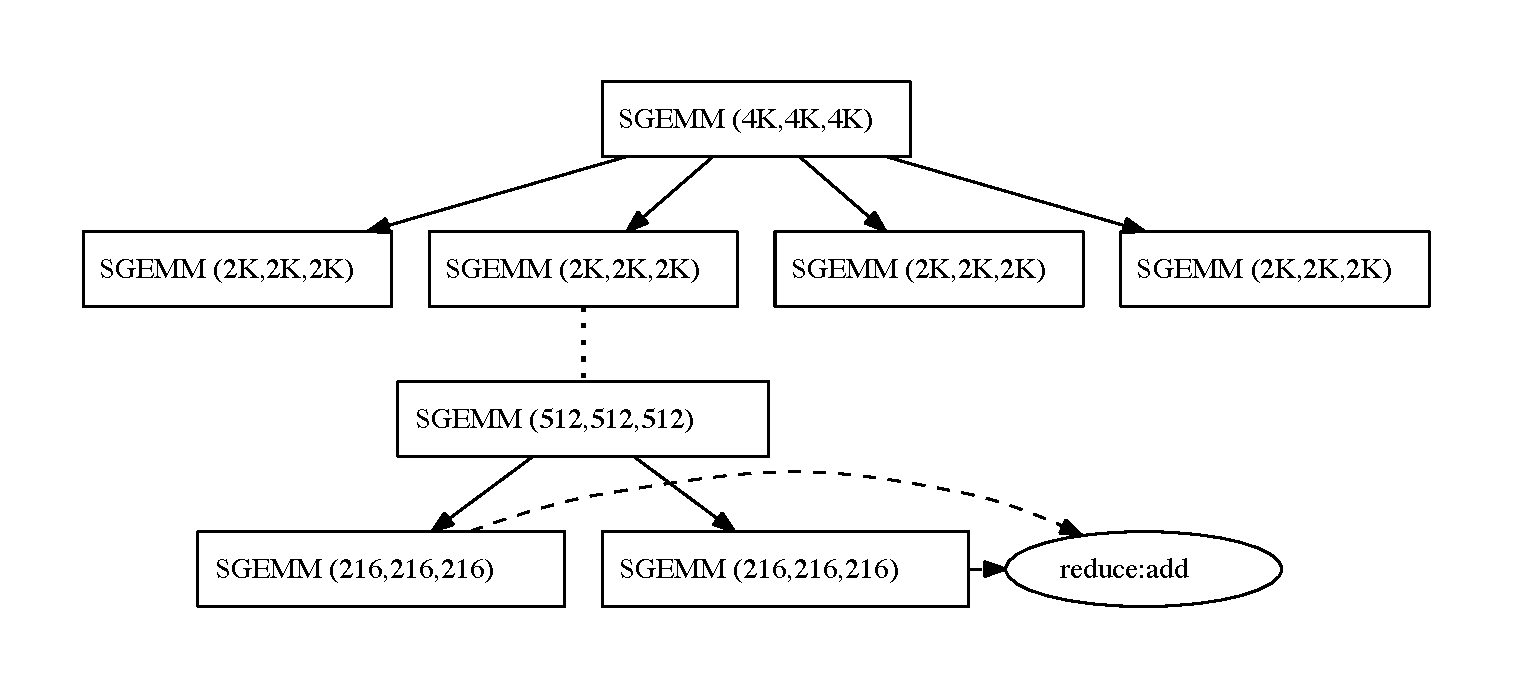
\includegraphics[width=3.6in]{../mmexample}
\caption{An illustration of recursively dividing SGEMM into subtasks, where
$M=P=N=4096$ and $K=2$. Note each task is divided into $K*K$ subtasks.
}
\label{fig:mmexample}
\end{figure}


\subsection{Example II: Pipeline Pattern}

\begin{figure}[hbt]
  \inputsrc{langpipe.cc}
  \caption{Source code of a pipeline pattern.}
  \label{fig:pipe:code}
\end{figure}

%Building blocks \textit{par} and \textit{reduce} to express execution.
\reffig{pipe:code} gives an example of pipeline processing similar to Streamit~\cite{ThiesKA02}.
In this example, the pipeline synthesizes four standalone functions.
Lines 1-16 define a full specialization of \code{TF\_pipeline}, which is the end
condition of recursion for definition \code{MYPIPE} at line 18-20.
Line 22 is an example of using \code{MYPIPE}. 
%\code{TF\_pipeline} is a TF class representing time-multiplex parallelism.

In execution time, each stage is running by a separate thread. Threads of
adjacent stages use \code{ReadViewMT} and \code{WriteViewMT} to synchronize.
%Asynchronous signals in ViewMTs provoke waiting stages and are used to mimic data-flow diagram.
As \reffig{viewmt} showing, \code{WriteViewMT} of a previous stage signals the
\code{ReadViewMT} of the next stage that data is ready.


%To leverage \code{TF\_pipeline}, programmers have to provide a full
%specialization template class. This is because \code{TF\_pipeline}
%only synthesizes functions and executes them in order, but does not
%know how to process the output.
%A full specialization of TF\_pipeline defines this behavior and is called at last.
%For example in \reffig{pipe}, line 2$\sim$21 is the case.
%Static entry at line 13 serves \code{TF\_pipeline} class. We spawn a thread to handle with the output 
%from the previous stage. Line 24$\sim$31 is a usage of \code{TF\_pipeline} with 4
%standalone functions. All the stages including our customized one are
%threads. It is noteworthy that each immediate stage, e.g.,
%\code{translate$<$Frn2Spn$>$}, has to follow type interfaces and
%define dependences.

\begin{figure}[tp]
  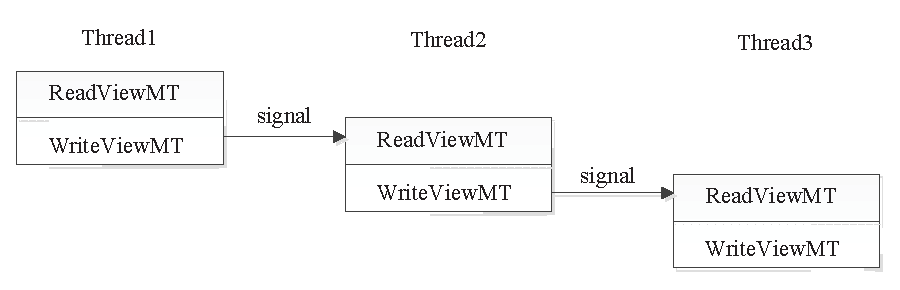
\includegraphics[width=3.6in]{../viewmt}
  \caption{Pipeline processing using ViewMTs. Access to a \code{ReadViewMT} is
  blocking until it is signaled. A stage sets its signal of \code{WriteViewMT}
after data processing is complete.}
  \label{fig:viewmt}
\end{figure}

In summary, the above two examples show that our approach can use uniform
language constructs to describe significantly different 
parallel patterns and execution models.


%meaning
\comment{
Our programming model facilitates the separation of roles in software
development. Algorithm-centric programmers are only concerned of algorithm
in conventional C/C++ form, as at line 45 of List 1 and line 8 of
List 2. On the other side,  system programmers knowing underlying
architectures are in charge of developing and
applying template classes to specialize tasks for the specific
targets. This separation not only simplifies the difficulties of writing and
tuning parallel programs, but also facilitates to develop effecient and
portable programs for various multicores.
}


%for sequoia's programming mode: 
%define recursive rules 
% for stream 's programming model:



\comment{
\subsection{Function Wrapper}
Function wrapper is an idiom in libvina. Our approach needs to manipulate
template functions according to their template arguments. However, a
template function is unaddressable until it is
instantiated. Thus programmers have to bind their template functions
to entries of classes.  Either static function or call operator
fuctions is approachable, but there is tradeoff to consider.
Static function need to predefine naming convention. 
For example, \code{TF\_hierarchy} use names \code{inner} and
\code{leaf} to call back. Call operator has unique form to invoke, so we leave it
as user interface, at expense of runtime
cost~\footnote{C++ does not allow overload call operator using static
function, therefore we have to generate an object to call it.}. Line 14
of \reffig{sgemm} is the case.
}

%Another restrict of function is that our
%template can only handle fixed form of function. \textit{i.e.} the
%function signature is triple form\footnote{function form: void (ARG0, ARG1,
% RESULT).We expect template alias in C++0x can releave this
%  retrict. } and parameter passing semantics is CBVR~\cite{dragonbook}.

